\subsection{Klassifizierungen}

Sei \(R\subseteq A\times A\) eine (homogene) Relation auf \(A\).

\subsubsection{Reflexivität}
Eine Relation \(R\) heisst \emph{reflexiv}, wenn jedes Element in Relation zu sich selbst steht:
\[\forall x\in A(xRx)\]
\begin{itemize}
    \item \(\{(a,a)\mid a\in A\}\subseteq R\).
    \item Im gerichteten Graphen hat jeder Knoten eine Kante zu sich selbst. Für jeden Wert \(x\in A\) gilt:
      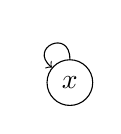
\begin{tikzpicture}[main/.style = {draw, circle}] 
        \node[main] (x) {$x$};
        \draw[->] (x) to [out=90,in=140,looseness=4] (x);
      \end{tikzpicture}
    \item In der Koordinatendarstellung enthält \(R\) die Winkelhalbierende \(y=x\).
\end{itemize}

\subsubsection{Symmetrie}
Eine Relation \(R\) heisst \emph{symmetrisch}, wenn für alle \(x,y\in A\) gilt:
\[
  \forall x,y\;(xRy\Rightarrow yRx).
\]
\begin{itemize}
  \item Symmetrie: zu jedem Pfeil im gerichteten Graph existiert der umgekehrte Pfeil. Für alle \(x,y\in A\) gilt:\\
    \begin{tikzpicture}[main/.style = {draw, circle}] 
      \node[main] (x) {$x$};
      \node[main] (y) [right=0.5cm of x] {$y$};
      \draw[<->] (x) to (y);
    \end{tikzpicture}
\end{itemize}

\subsubsection{Antisymmetrie}
Eine Relation \(R\) heisst \emph{antisymmetrisch}, wenn für
alle \(x,y\in A\) gilt:
\[
    \forall x,y\;(xRy\land yRx\Rightarrow x=y).
\]
\begin{itemize}
  \item Antisymmetrie: es gibt keine zwei verschiedenen Knoten, die wechselseitig verbunden sind.
    Für alle \(x,y\in A, x\neq y\) gilt:\\
    \begin{tikzpicture}[main/.style = {draw, circle}] 
      \node[main] (x) {$x$};
      \node[main] (y) [right=0.5cm of x] {$y$};
      \draw[->] (x) to (y);
    \end{tikzpicture}
  \item Symmetrie spiegelt die Koordinatendarstellung an der Geraden \(y=x\).
\end{itemize}

\subsubsection{Transitivität}
Eine Relation \(R\) heisst \emph{transitiv}, wenn für jeden endlichen Pfad ein direkter Pfeil existiert. Für alle \(x,y,z\in A\) gilt:
\[
  \forall x,y,z\;(xRy\land yRz\Rightarrow xRz).
\]
\begin{itemize}
    \item Im gerichteten Graphen: Aus \(x\to y\) und \(y\to z\) folgt \(x\to z\). Für alle \(x,y,z\in A\) gilt:\\
      \begin{tikzpicture}[main/.style = {draw, circle}] 
        \node[main] (x) {$x$};
        \node[main] (y) [right=0.5cm of x] {$y$};
        \node[main] (z) [right=0.5cm of y] {$z$};
        \draw[->] (x) to (y);
        \draw[->] (y) to (z);
        \draw[->, dashed] (x) to [bend left] (z);
      \end{tikzpicture}
\end{itemize}

\subsubsection{Totalität und Eindeutigkeit}
Sei \(R\subseteq A\times B\) eine Relation von \(A\) nach \(B\) mit
\begin{itemize}
  \item \textbf{Linksvollständig / linkstotal:} \(\mathrm{dom}(R)=A\) (jede \(x\in A\) hat ein Bild).
  \item \textbf{Rechtsvollständig / rechtstotal:} \(\mathrm{im}(R)=B\) (jedes \(y\in B\) wird erreicht).
  \item \textbf{Linkseindeutig:} \(\forall x_1,x_2,y\;(x_1Ry\land x_2Ry\Rightarrow x_1=x_2)\).
  \item \textbf{Rechtseindeutig:} \(\forall x,y_1,y_2\;(xRy_1\land xRy_2\Rightarrow y_1=y_2)\).
\end{itemize}
